\documentclass[a4paper,11pt]{article}

\usepackage[utf8]{inputenc}
\usepackage[italian]{babel}
\usepackage[sfdefault]{roboto}
\usepackage{layaureo} % reduce margins
\usepackage{url}
\usepackage{hyperref}
\usepackage{graphicx}
\usepackage{float}
\usepackage{alertmessage}

% Setup
\hypersetup{hidelinks}
\hyphenation{knolleary}
\hyphenation{crankyoldgit}

% Document
\begin{document}
\title{IR Extender}
\author{Davide Pizzoli \\ Stefano Zenaro}
\date{Aprile 2022}

\pagenumbering{gobble}

% Title
\begin{titlepage}
  \maketitle
  \thispagestyle{empty}
\end{titlepage}

% Table of contents
\tableofcontents
\addcontentsline{toc}{section}{Indice}
\clearpage

\pagenumbering{arabic}

% Contents
\section{Descrizione}

    L'IR Extender permette di controllare da remoto dispositivi infrarossi a lunga distanza attraverso Internet.

    \begin{figure}[H]
      \centering
      \includegraphics[width=\textwidth,height=\textheight,keepaspectratio]{assets/ir_extender}
      \caption{IR Extender}
    \end{figure}

    Il sistema è composto da 3 componenti:
    \begin{itemize}
      \item Ricevitore: riceve un segnale infrarossi e lo comunica al Broker MQTT attraverso un messaggio
      \item Broker MQTT: permettere lo scambio di messaggi tra Ricevitore e Trasmettitore
      \item Trasmettitore: riceve il messaggio dal Broker MQTT e propaga il segnale infrarossi verso il dispositivo da controllare
    \end{itemize}

    \alertinfo{Ricevitore e trasmettitore possono essere collegati alla stessa rete \mbox{Wi-Fi} oppure a due reti \mbox{Wi-Fi} differenti.}

\section{Configurazione}

    \subsection{Prerequisiti}

    Componenti elettronici:
    \begin{itemize}
      \item IR Receiver
      \item IR Transmitter
      \item ESP32 * 2
      \item Jumpers * 6
    \end{itemize}

    \begin{samepage}
      \noindent
      Servizi cloud:
      \begin{itemize}
        \item Broker MQTT (es. \href{https://www.hivemq.com/}{HiveMQ})
      \end{itemize}
    \end{samepage}

    \begin{samepage}
      \noindent
      Librerie:
      \begin{itemize}
        \item Espressif 32: supporto alla board ESP32.
        \item PubSubClient (knolleary): libreria per la comunicazione attraverso il protocollo MQTT
        \item IRremoteESP8266 (crankyoldgit): libreria per inviare/ricevere segnali infrarossi
      \end{itemize}
    \end{samepage}

    \subsection{Broker MQTT (HiveMQ)}
    \label{subsec:Broker}

    Per permettere la comunicazione tra ricevitore e trasmettitore è prima necessario configurare il broker MQTT:

    \begin{enumerate}
      \item \href{https://console.hivemq.cloud/}{Registrarsi su HiveMQ}
      \item Creare un nuovo \emph{Cluster}
        \begin{figure}[H]
          \centering
          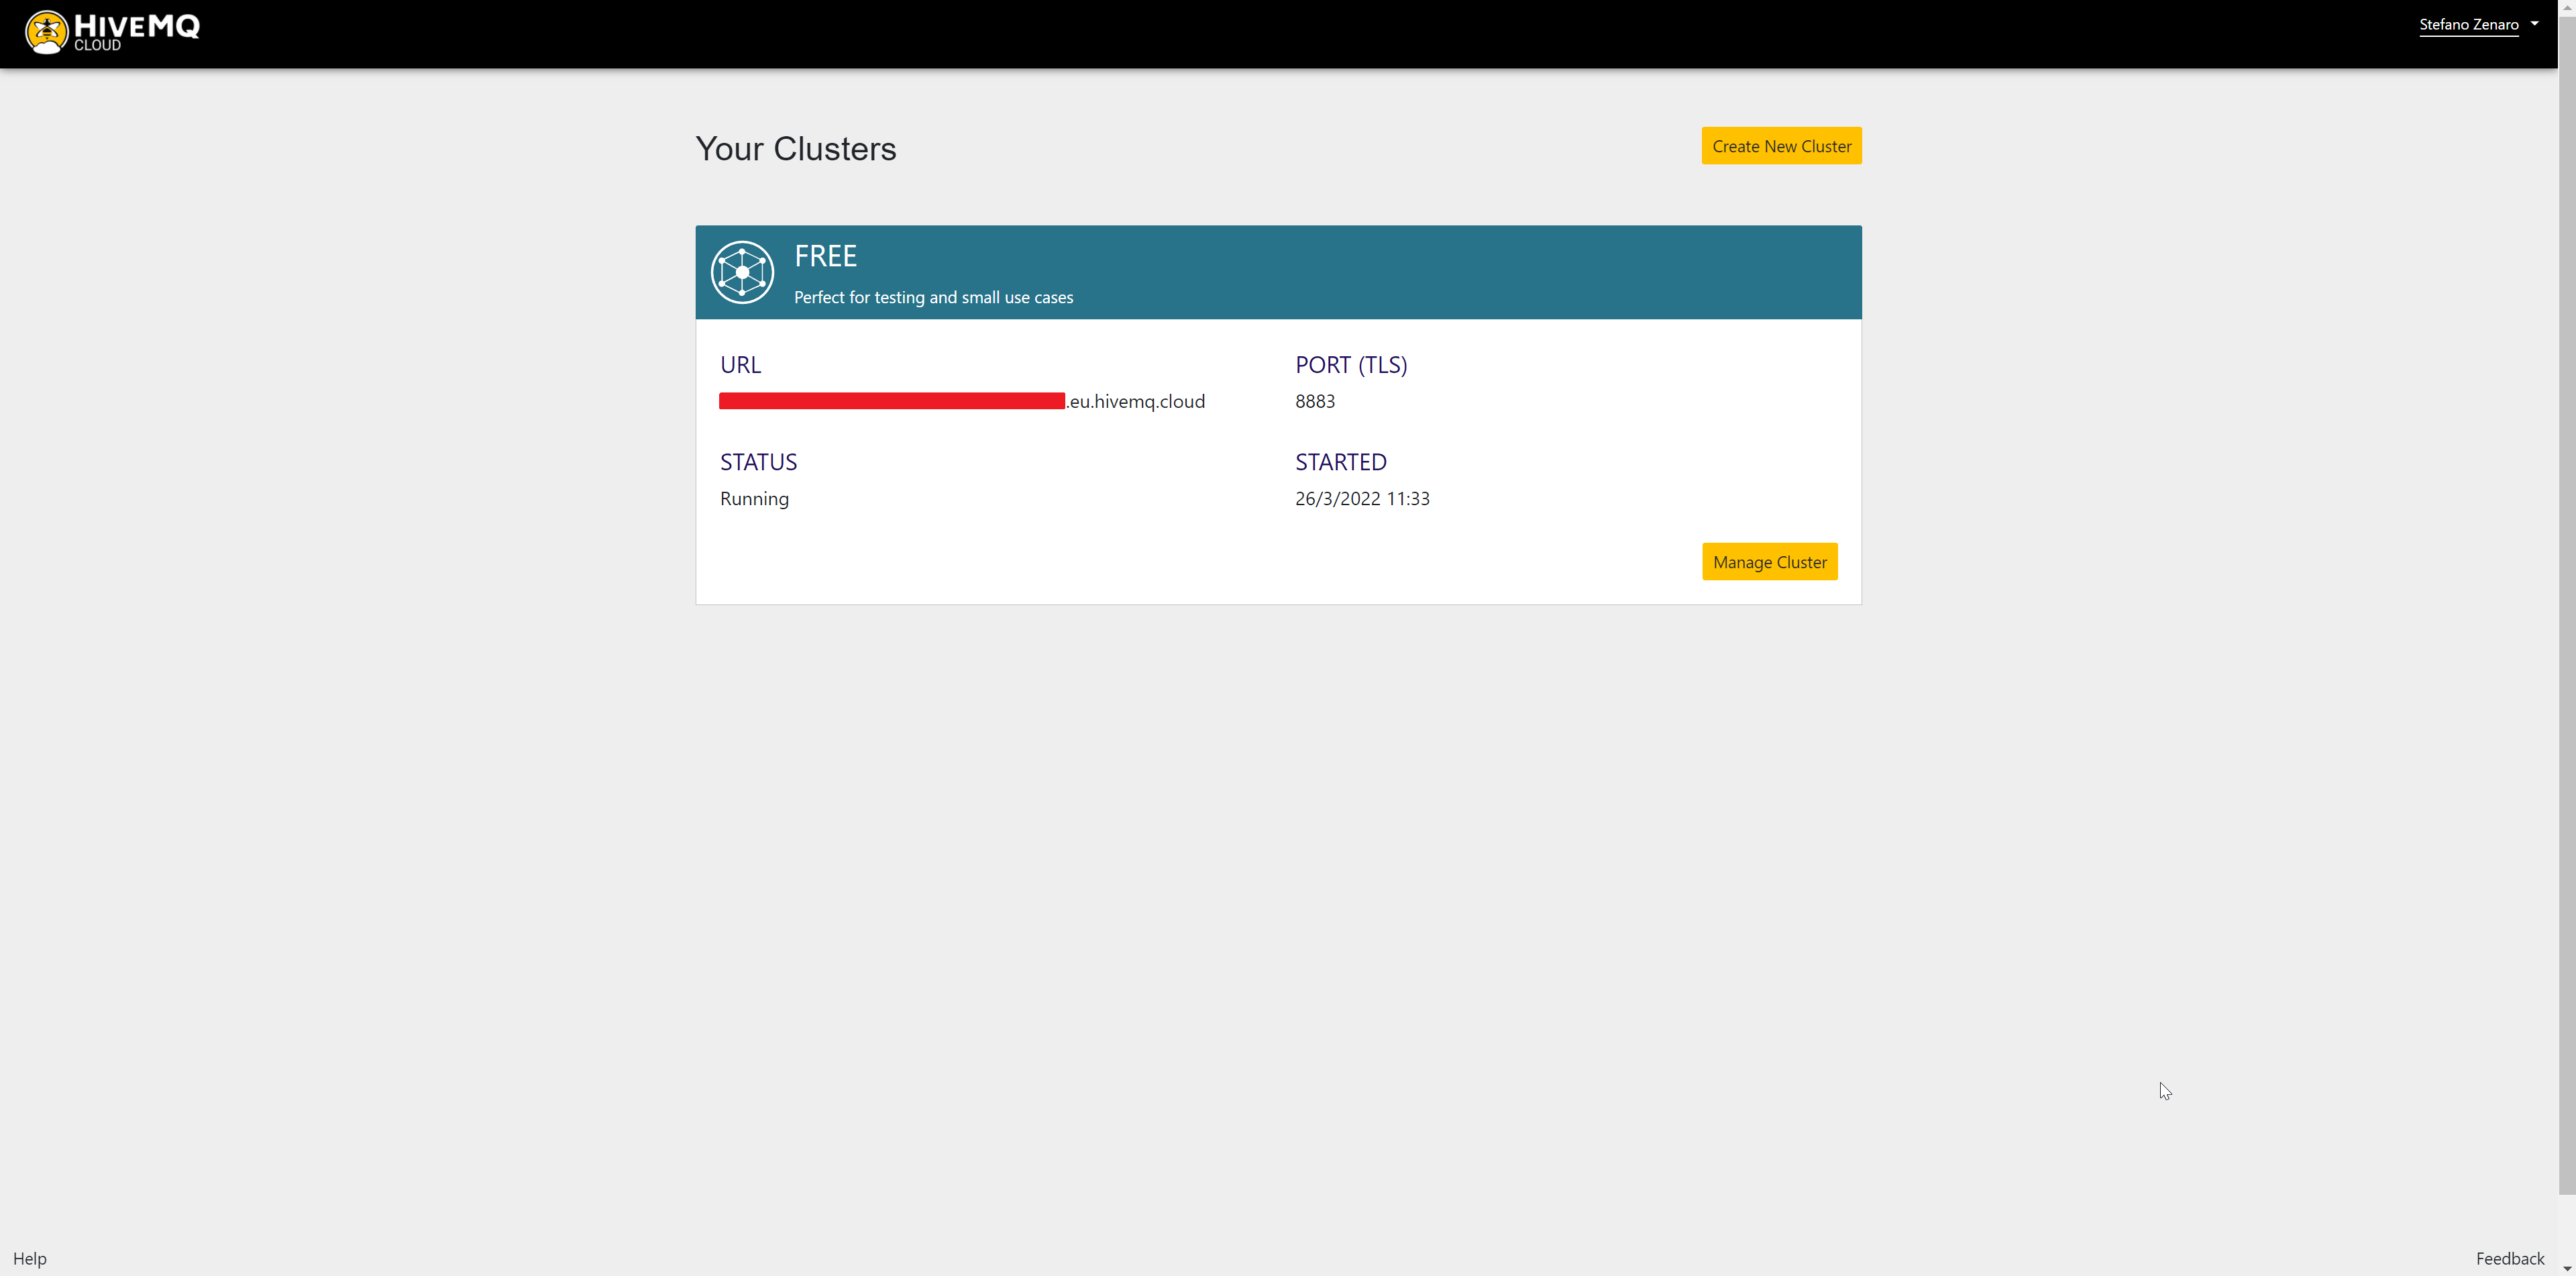
\includegraphics[width=0.8\textwidth,height=\textheight,keepaspectratio]{assets/hivemq_clusters}
        \end{figure}

        Salvarsi l'\emph{URL} del Cluster, che sarà utilizzato per configurare il Ricevitore e il Trasmettitore.

      \item Cliccare su \emph{Manage cluster}
        \begin{figure}[H]
          \centering
          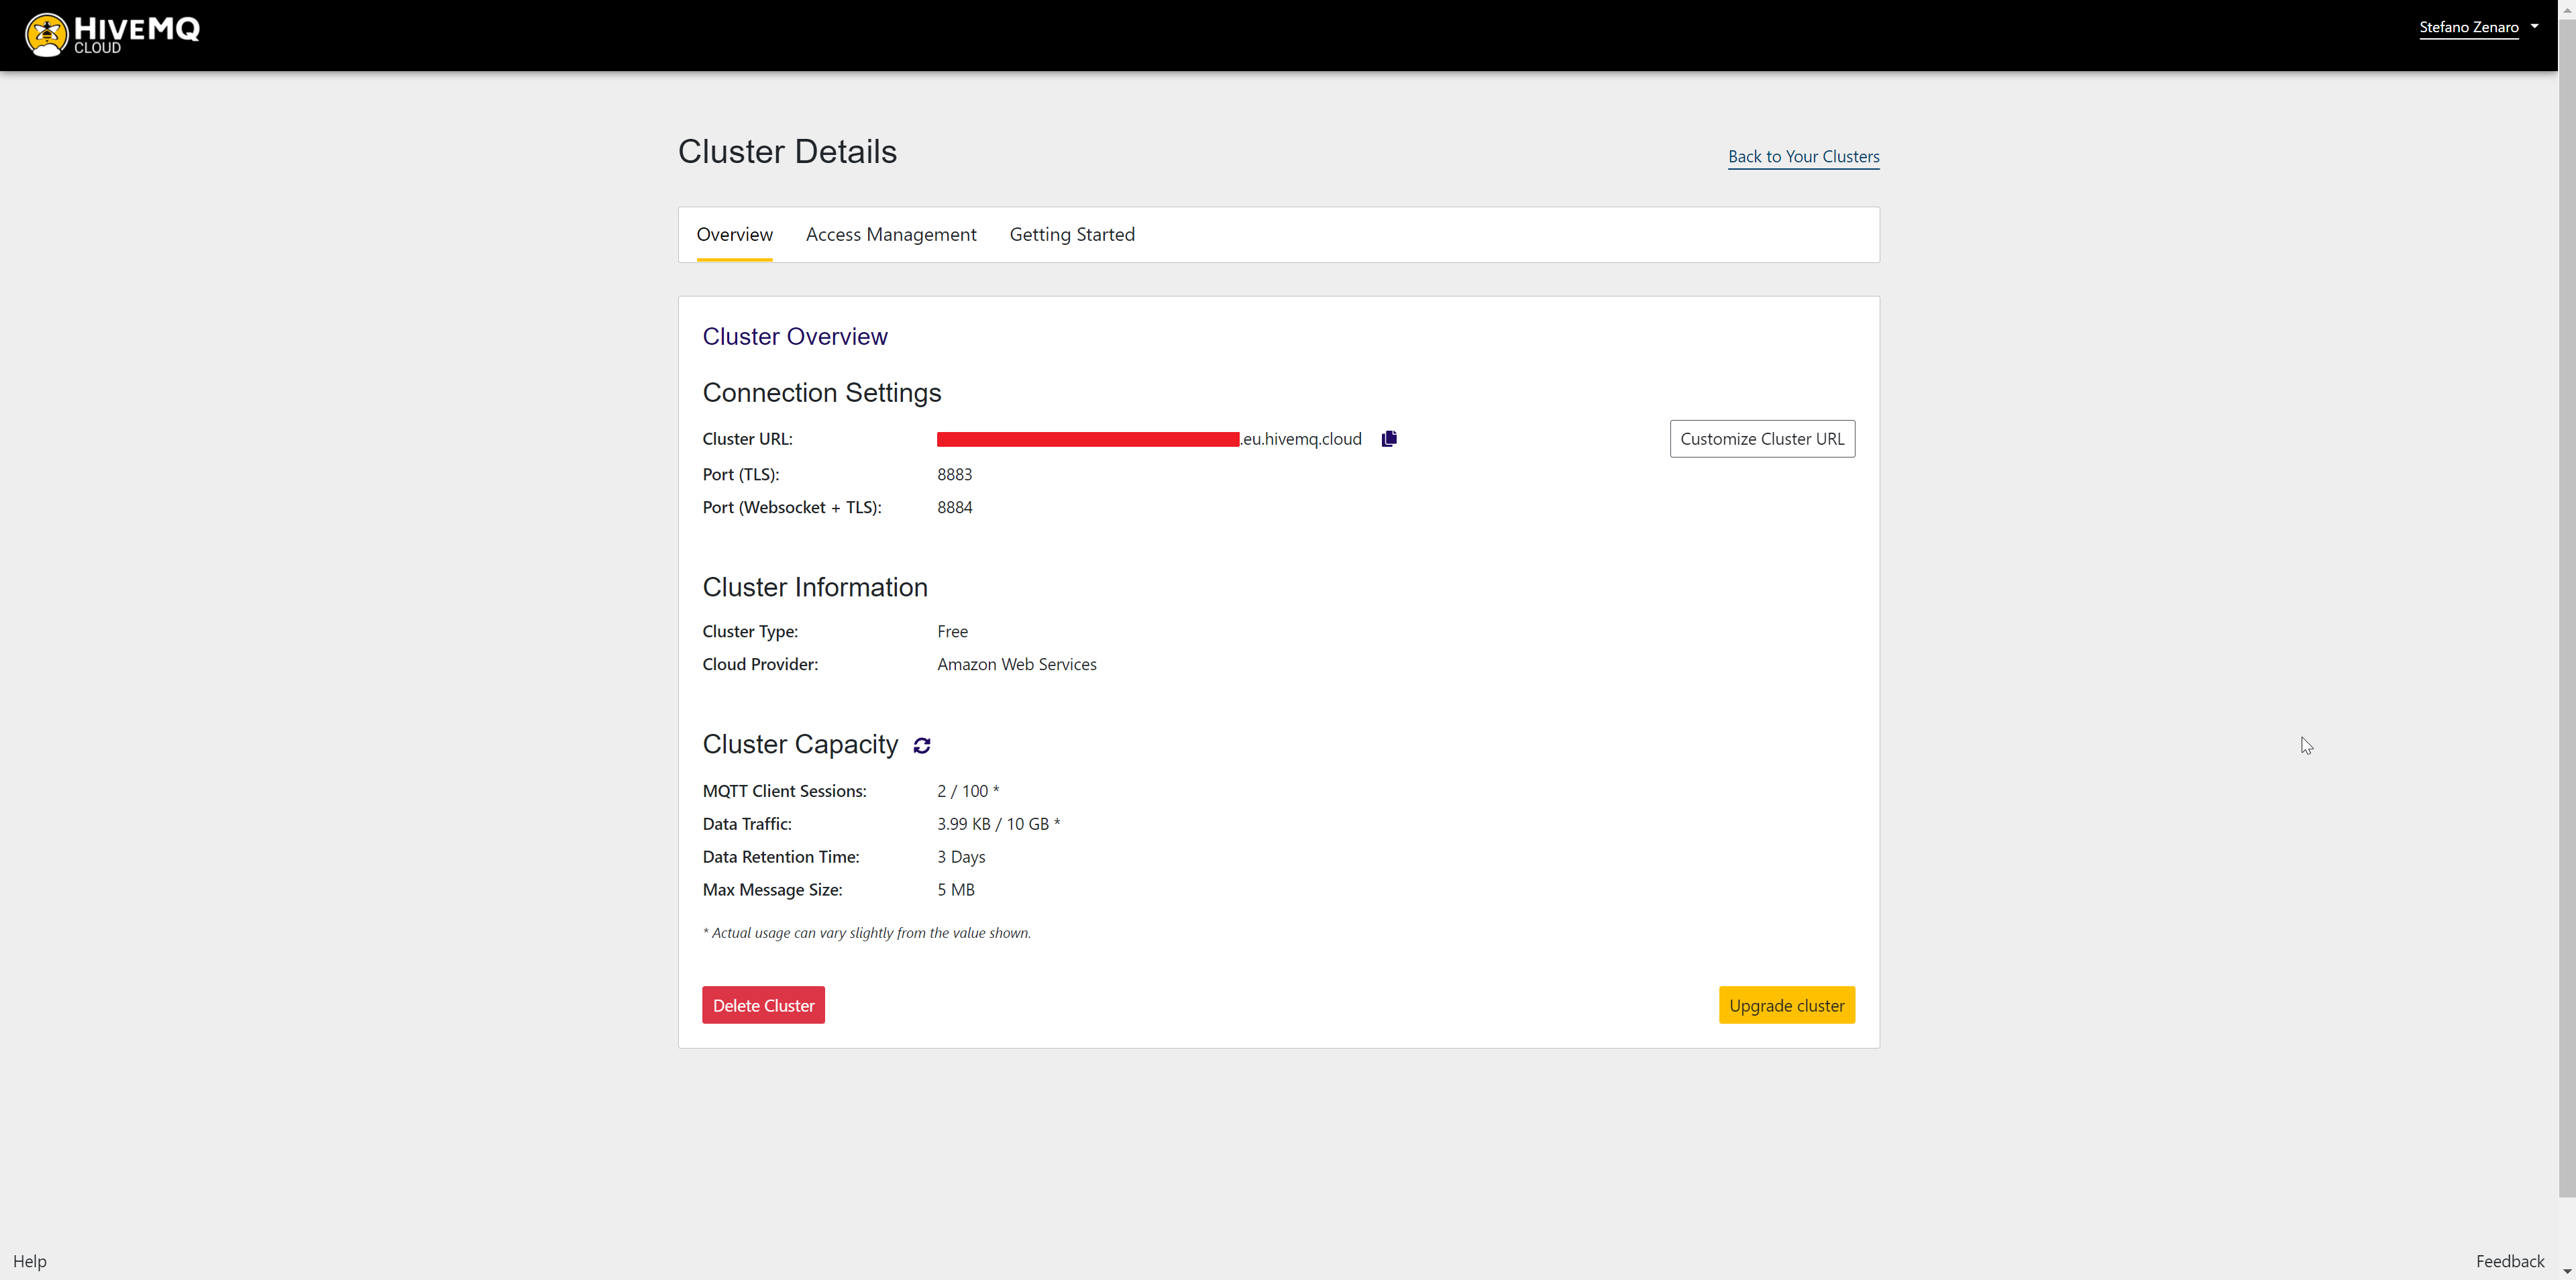
\includegraphics[width=0.8\textwidth,height=\textheight,keepaspectratio]{assets/hivemq_clusterdetails}
        \end{figure}

      \item Nella sezione \emph{Access Management} aggiungere delle credenziali di accesso al \emph{Cluster}
        \begin{figure}[H]
          \centering
          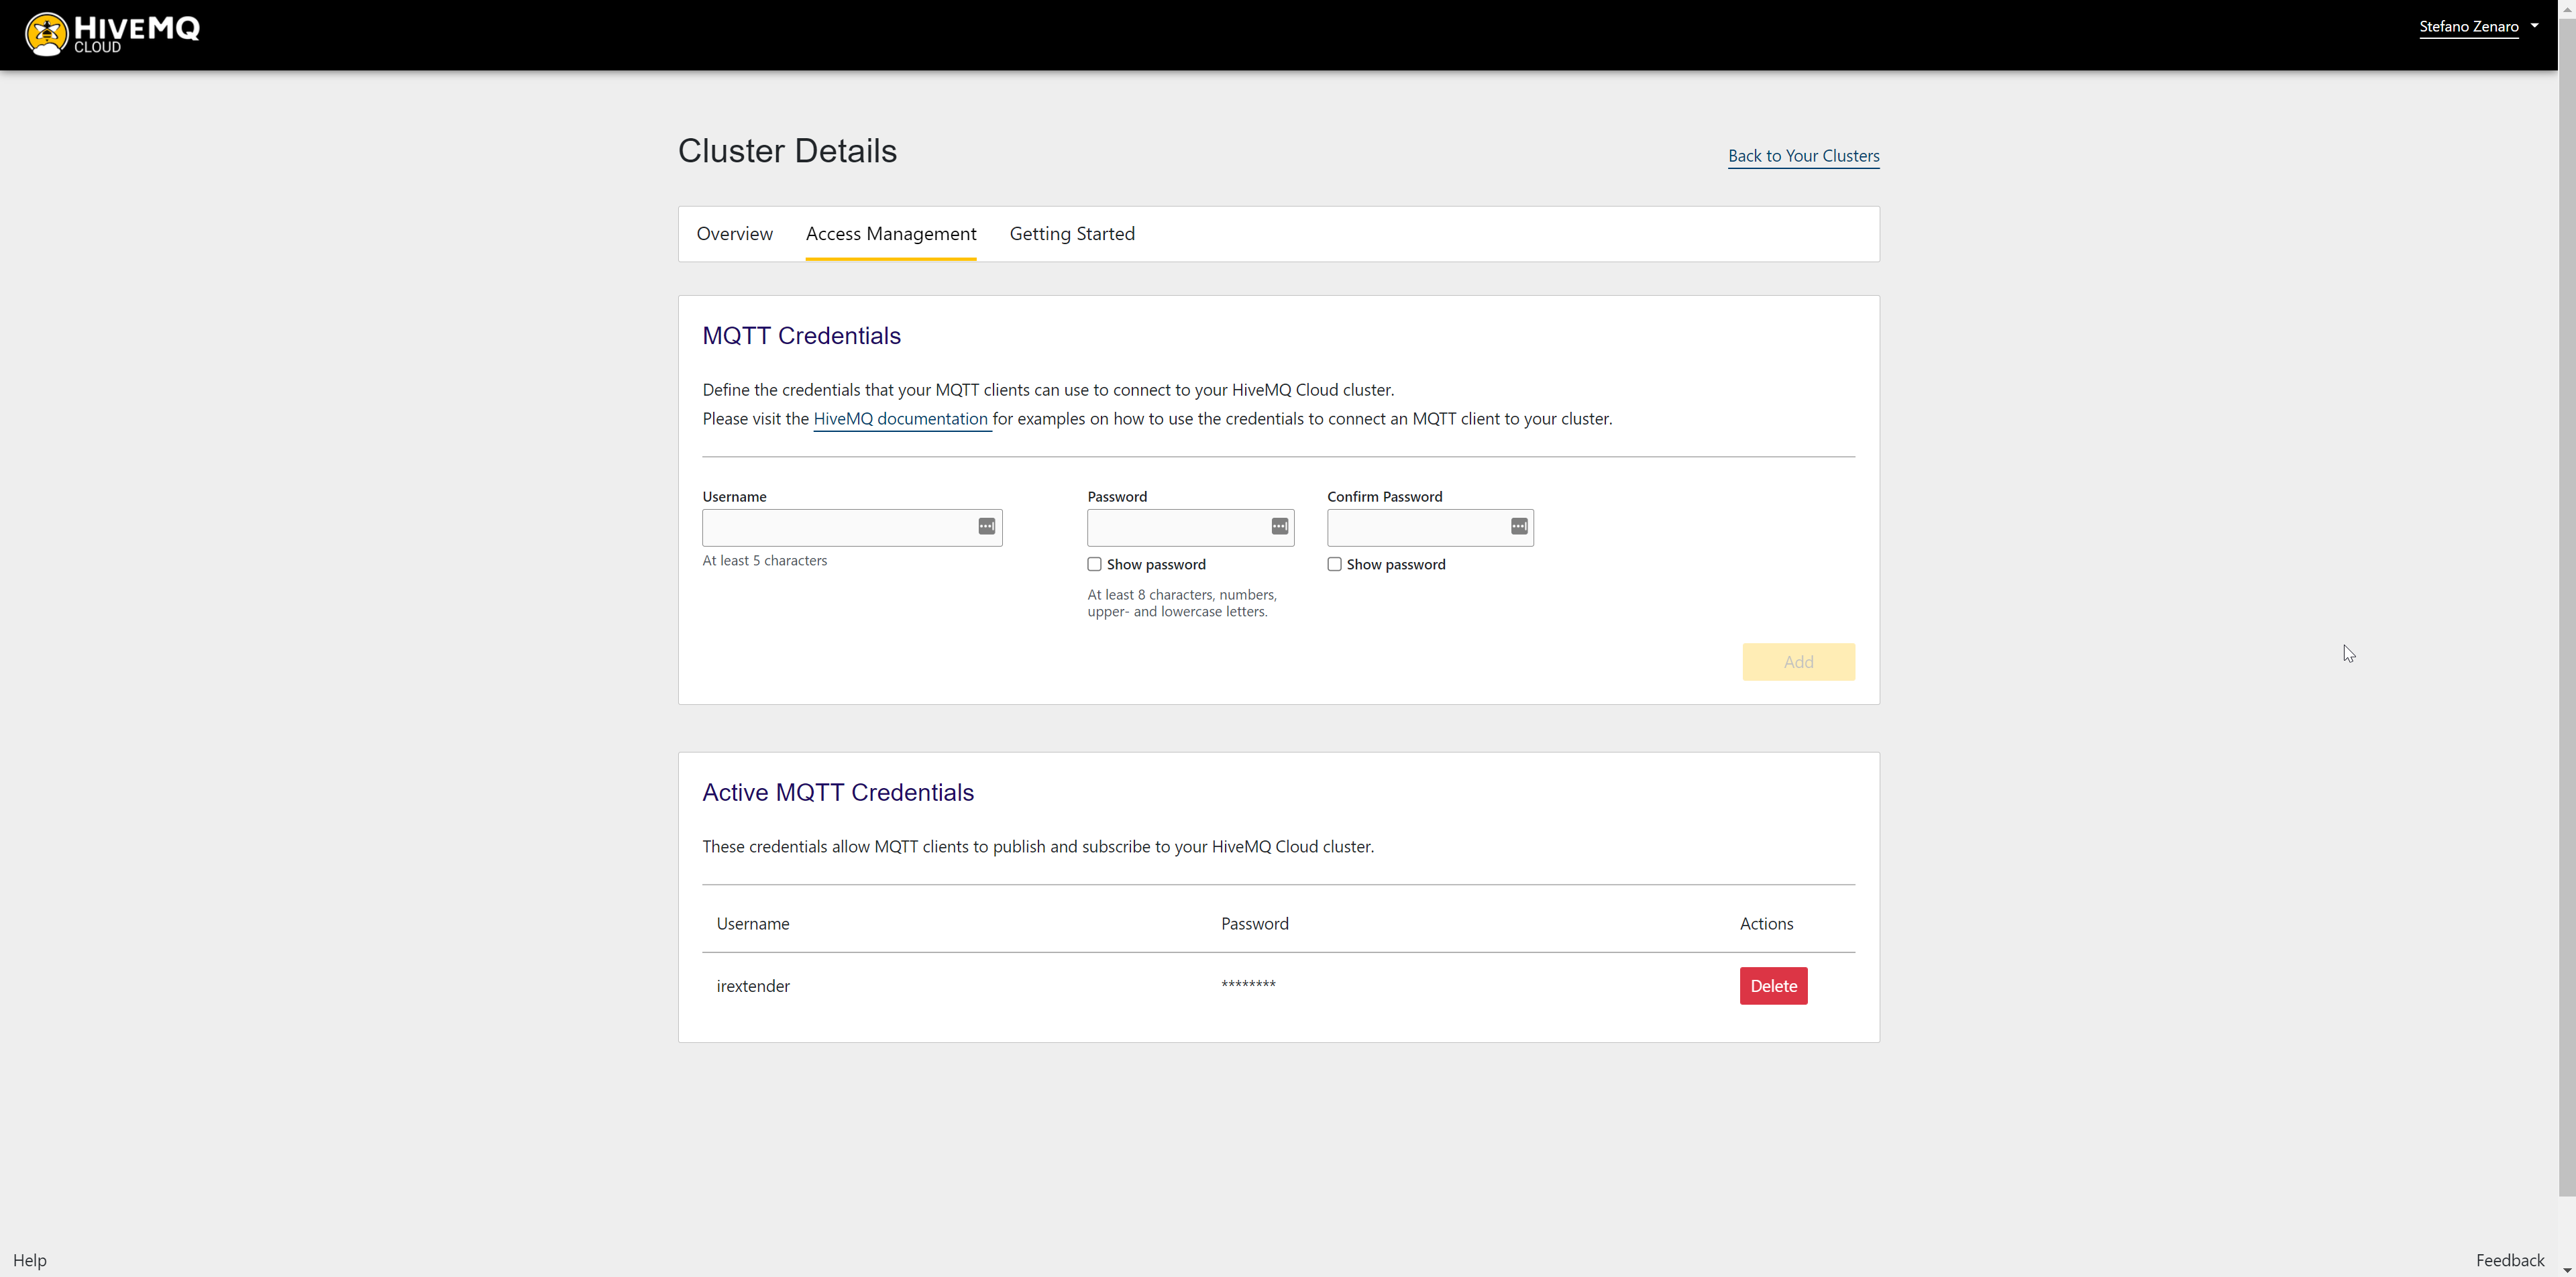
\includegraphics[width=0.8\textwidth,height=\textheight,keepaspectratio]{assets/hivemq_access_management}
        \end{figure}

    \end{enumerate}

    \subsection{Ricevitore}
    \label{subsec:receiver}

    Il dispositivo ricevitore si occupa di:

    \begin{enumerate}
      \item Ricevere un segnale infrarossi da un telecomando
      \item Inviare l'informazione del segnale infrarossi, utilizzando la rete Wi-Fi, con il protocollo MQTT al Broker MQTT
    \end{enumerate}

    Per predisporre il ricevitore a ricevere segnali infrarossi e ad inoltrarli al broker MQTT occorre:

    \begin{itemize}
      \item Collegare il ricevitore infrarossi all'ESP32 (figura~\ref{fig:circuito_ricevitore}):
        \begin{itemize}
          \item Il ground del ricevitore al pin GND;
          \item VCC al pin 3V3;
          \item data/signal al pin G13/13;
        \end{itemize}

        \alertinfo{Assicurarsi di collegare correttamente l'alimentazione e il cavo dati verificando il pinout del ricevitore infrarossi e dell'ESP32. I pin potrebbero essere posizionati diversamente (da scheda a scheda, da sensore a sensore) rispetto allo schema nella figura~\ref{fig:circuito_ricevitore}.}

      \item Aprire la cartella \texttt{receiver/src}
      \item Rinominare il file \texttt{secrets.h.sample} in \texttt{secrets.h} e aprirlo
      \item Inserire i dati di accesso della rete WiFi e del \hyperref[subsec:Broker]{Broker MQTT}
      \item Caricare il programma sull'ESP32
    \end{itemize}

    \begin{figure}[H]
      \centering
      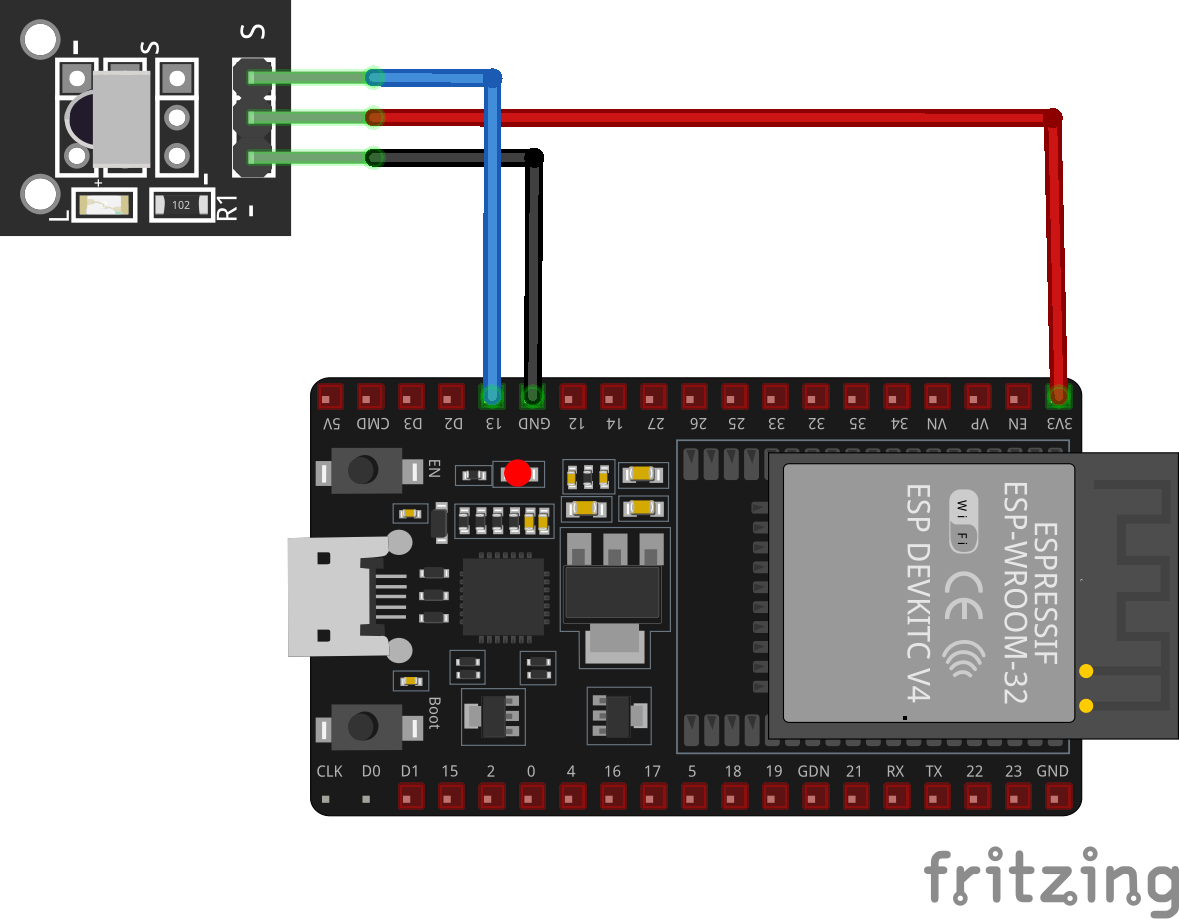
\includegraphics[width=0.5\textwidth,height=\textheight,keepaspectratio]{assets/receiver_fritzing}
      \caption{Circuito Ricevitore}
      \label{fig:circuito_ricevitore}
    \end{figure}


    \subsection{Trasmettitore}
    \label{subsec:transmitter}

    Il dispositivo trasmettitore si occupa di:

    \begin{enumerate}
      \item Ricevere l'informazione dal Broker MQTT
      \item Inviare il segnale ricevuto tramite il trasmettitore infrarossi
    \end{enumerate}

    Per predisporre il trasmettitore a ricevere messaggi dal broker MQTT e di propagare segnali infrarossi occorre:

    \begin{itemize}
      \item Collegare il trasmettitore infrarossi all'ESP32 (figura~\ref{fig:circuito_trasmettitore}):
        \begin{itemize}
          \item Il ground del trasmettitore al pin GND;
          \item VCC al pin 3V3;
          \item data/signal al pin G12/12;
        \end{itemize}

        \alertinfo{Assicurarsi di collegare correttamente l'alimentazione e il cavo dati verificando il pinout del trasmettitore infrarossi e dell'ESP32. I pin potrebbero essere posizionati diversamente (da scheda a scheda, da sensore a sensore) rispetto allo schema nella figura~\ref{fig:circuito_trasmettitore}.}

      \item Aprire la cartella \texttt{transmitter/src}
      \item Rinominare il file \texttt{secrets.h.sample} in \texttt{secrets.h} e aprirlo
      \item Inserire i dati di accesso della rete WiFi e del \hyperref[subsec:Broker]{Broker MQTT}
      \item Caricare il programma sull'ESP32
    \end{itemize}

    \begin{figure}[H]
      \centering
      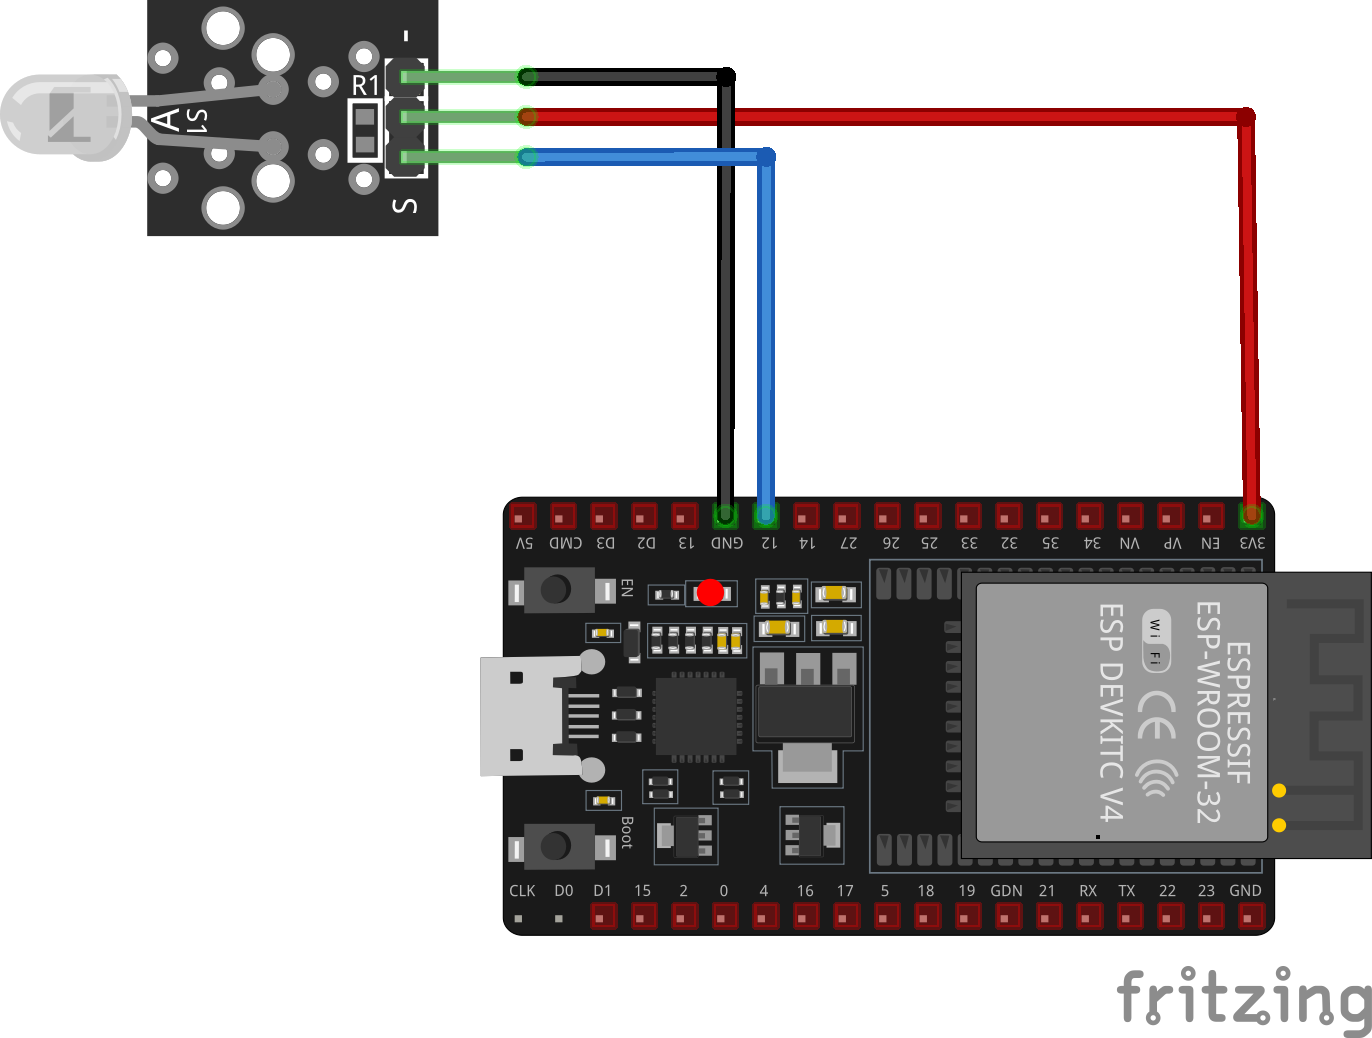
\includegraphics[width=0.5\textwidth,height=\textheight,keepaspectratio]{assets/transmitter_fritzing}
      \caption{Circuito Trasmettitore}
      \label{fig:circuito_trasmettitore}
    \end{figure}

\section{Scelte progettuali}

    \subsection{Protocollo messaggio MQTT}

    La libreria che interpreta i dati rilevati dal sensore infrarossi può rilevare 3 tipi di protocolli:
    \begin{itemize}
      \item Protocollo a stati: composto da più di un valore. Usato, ad esempio, per i condizionatori.
      \item Protocollo semplice: formato da un singolo valore.
      \item Protocollo sconosciuto: non è stato possibile rilevare il protocollo. Verranno inviati tutti i valori rilevati durante la lettura.
    \end{itemize}

    \noindent
    Per gestire le 3 casistiche si è realizzato un protocollo per il messaggio MQTT:
    \smallskip

    Per i protocolli a stati verrà inviata una stringa con il formato:

    \begin{verbatim}
      <protocol>|<length>|<value1>,<value2>,...|<size>
    \end{verbatim}

    Dove:
    \begin{itemize}
      \item "protocol" è un identificativo del protocollo rilevato dal sensore IR
      \item "length" è il numero di valori "valueX"
      \item "valueX" sono valori \emph{raw} letti dal sensore IR
      \item "size" (in bit) verrà usato dal metodo send() con il trasmettitore IR
    \end{itemize}

    \bigskip

    \begin{samepage}
      Per i protocolli semplici verrà inviata una stringa con il formato:

      \begin{verbatim}
        <protocol>|1|<value>|<size>
      \end{verbatim}

      Dove:
      \begin{itemize}
        \item "protocol" è un identificativo del protocollo rilevato dal sensore IR
        \item "1" indica che c'è un solo valore letto
        \item "value" è il valore letto. Verrà usato dal metodo send() con il trasmettitore IR
        \item "size" (in bit) verrà usato dal metodo send() con il trasmettitore IR
      \end{itemize}
    \end{samepage}

    \bigskip

    \begin{samepage}
      Per i protocolli non riconosciuti verrà inviata una stringa con il formato:

      \begin{verbatim}
        -1|<length>|<value1>,<value2>,...|-1
      \end{verbatim}

      Dove:
      \begin{itemize}
        \item "-1" indica che il protocollo non è stato riconosciuto
        \item "length" è il numero di valori "valueX"
        \item "valueX" sono valori raw letti dal sensore IR. Questi valori verranno trasmessi dal metodo sendRaw() con il trasmettitore IR
        \item "-1" (size) indica "non applicabile" poichè il protocollo non richiede state[]
      \end{itemize}
    \end{samepage}

\section{Limitazioni trovate nello svolgimento del progetto}

    \subsection{Differenze nei segnali infrarossi per ogni produttore}

    Ogni produttore di dispositivi che utilizzano segnali ad infrarossi, crea un proprio protocollo per la decodifica dei segnali.
    Le differenze possono essere termini di pause tra un dato e l'altro, intensità e frequenze.

    Nel caso di un protocollo non riconosciuto il segnale verrà comunque letto come segnale grezzo e inviato, ma non è garantito il corretto funzionamento.

    \bigskip
    \noindent
    Una lista dei protocolli supportati è disponibile sulla \href{https://github.com/crankyoldgit/IRremoteESP8266/blob/master/SupportedProtocols.md}{pagina ufficiale della libreria IRremoteESP8266}

\section{Troubleshooting}

    \subsection{Segnale infrarossi non rilevato}

    Per non rilevare troppo rumore è stata modificata la dimensione del buffer di memoria usato per memorizzare i dati letti dal sensore infrarossi.

    È possibile cambiare la dimensione del buffer dal file \texttt{receiver/src/main.hpp} modificando la variabile "BUFFER\_SIZE": riducendo il valore aumenterà la velocità di lettura 
    del sensore infrarossi permettendo di leggere (dal sensore) e trasmettere (al broker MQTT) più valori ma aumentando la probabilità di rilevare rumore e quindi di ottenere dati inutilizzabili dal trasmettitore.
    Aumentando la dimensione del buffer rallenterà sensibilmente la velocità del sistema con il rischio che il sensore infrarossi non riuscirà a rilevare dati sufficienti per poterli spedire al broker MQTT.

\clearpage

% List of figures
\listoffigures
\addcontentsline{toc}{section}{\listfigurename}

\end{document}
